\section{Standard Model mapping and the top-quark criterion}\label{rep:h-smmap}

The Standard Model enters the Higgs calculation through the couplings $(\lambda,g_2,g_Y,g_3,y_t)$ at the nodes $\mu(\tau)$ of Eq.~(\ref{eq:rb-mutau}).
We map the threshold of Secs.~\ref{rep:h-reduced}--\ref{rep:h-survival} to the top-quark mass with three-loop Standard Model running and next-to-next-to-leading-order (NNLO) matching, computed with our own code (assumption (A2) of Sec.~\ref{rep:setup}).
With $m_t$ the top-quark pole mass and $\mtbar\equiv\mtbar(\mtbar)$ the $\MSbar$ mass of assumption (A7), the result is
\begin{equation}
P_1>\tfrac12 \;\Longleftrightarrow\; m_t<172.96~\mathrm{GeV}
\quad\bigl[\,\bar m_t<163.16~\mathrm{GeV}\,\bigr], %
\label{eq:rb-criterion}
\end{equation}
for $\alpha_s(M_Z)=0.1180$; the Standard Model theory error is $\pm0.10\GeV$ for $m_t$ and $\pm0.07\GeV$ for $\mtbar$, and $\alpha_s\pm0.0009$ moves the bound by $\pm0.35\GeV$ ($\pm0.25\GeV$ for $\mtbar$). %
The levels $\Pone=0.9$ and $0.1$ give $m_t=172.50$ and $173.42\GeV$ ($\mtbar=162.73$ and $163.60\GeV$). %
The criterion lies $m_c-m_0=\mcMinusMzero\GeV$ above the line $\lambda(\mub)=0$, at $m_0=171.09\GeV$, which in turn lies $0.10\GeV$ above the absolute-stability line of the same mapping, $m_t=170.99\GeV$, computed for this report (Sec.~\ref{sec:rb-absstab}). %
We also show that the larger scale dependence of the tadpole-including organization of the fixed-order matching comes from same-sign two-loop logarithms in the $G_F$ scheme rather than from tadpoles.
We use $\MSbar$ couplings with $g_Y=g'=\sqrt{3/5}\,g_1^{\rm GUT}$ and $V=\lambda(|H|^2-v^2/2)^2$, and $\mub=\MPbar/722=3.3726\times10^{15}\GeV$. %

\subsection{Matching at the top-quark mass}
\label{sec:rb-sm-matching}

At $\mu_0=m_t$ we take the reference model of SMDR~1.3~\cite{Martin:2019lqd}, which uses the tadpole-free pure $\MSbar$ scheme with inputs $(G_F,\alpha,M_Z,M_h,m_t,\alpha_s)$, complete two-loop and leading three-loop threshold corrections, and four-loop QCD for the top mass.
We move it to the desired $(m_t,\alpha_s,M_h)$ with the linear slopes of Ref.~\cite{Buttazzo:2013uya}.
Across the reference models of several releases this shift reproduces $\lambda$, $y_t$, and $g_3$ at $m_t$ to $2.3\times10^{-5}$, $4.9\times10^{-6}$, and $3.8\times10^{-6}$, and the quartic at $\mub$ to $3.9\times10^{-5}$, which is $0.006\GeV$ in $m_t$. %
We also compiled SMDR and fitted the inputs directly.
At $\mu=m_t$ the compiled fit and the shifted reference model differ by at most $3.0\times10^{-6}$ in $\lambda$ and $7.4\times10^{-6}$ in $y_t$, and in the hazard the two give critical masses within $0.005\GeV$. %
A fit with all evaluation scales at their default values reproduces every $\MSbar$ parameter of the reference model to $8\times10^{-13}$. %

\subsection{Running to the bounce scale}
\label{sec:rb-sm-running}

The $\beta$ functions are generated automatically from the SMDR source: complete three-loop Standard Model running~\cite{Mihaila:2012fm,Bednyakov:2012rb,Bednyakov:2012en,Bednyakov:2013eba,Chetyrkin:2012rz,Chetyrkin:2013wya}, four-loop gauge couplings~\cite{Bednyakov:2015ooa,Zoller:2015tha,Davies:2019onf}, the leading four-loop QCD terms of $y_t$ and $\lambda$~\cite{Chetyrkin:1997dh,Vermaseren:1997fq,Martin:2015eia,Chetyrkin:2016ruf}, and five-loop QCD for $g_3$ and $y_t$~\cite{Baikov:2016tgj,Herzog:2017ohr,Baikov:2014qja}.
For orientation, the one-loop parts are
\begin{align}
16\pi^2\frac{dg_2}{d\ln\mu}&=-\frac{19}{6}g_2^3,\qquad 16\pi^2\frac{dg_Y}{d\ln\mu}=\frac{41}{6}g_Y^3,\qquad 16\pi^2\frac{dg_3}{d\ln\mu}=-7g_3^3,\nonumber\\
16\pi^2\frac{dy_t}{d\ln\mu}&=y_t\Bigl(\frac92y_t^2-8g_3^2-\frac94g_2^2-\frac{17}{12}g_Y^2\Bigr),
\label{eq:rb-beta1}
\end{align}
and $\beta_\lambda^{(1)}$ of Eq.~(\ref{eq:rb-betalam}); the term $-6y_t^4$ drives $\lambda$ negative at intermediate scales for the measured masses, and the decrease of $y_t$ (through $g_3$) makes $\lambda(\mu)$ turn up again at high scales~\cite{Degrassi:2012ry,Buttazzo:2013uya}; with our inputs the minimum lies near $5\times10^{17}\GeV$ (Sec.~\ref{sec:rb-absstab}). %
Light Yukawa couplings below $y_b$ are set to zero, which changes $\lambda$ by less than $10^{-6}$. %
A second implementation, copied by hand from the appendix of Ref.~\cite{Buttazzo:2013uya}, agrees term by term: to $4\times10^{-15}$ at one and two loops and for the three-loop gauge terms, and to $3.2\times10^{-6}$ ($y_t$) and $5.9\times10^{-5}$ ($\lambda$) at three loops, the rounding of the $\zeta_3$ coefficients in that appendix. %
Our running reproduces the published SMDR running up to $10^{19}\GeV$ with $|\Delta\lambda|\le9\times10^{-7}$, and an independent conversion of the same $\beta$ functions to Wolfram Language gives $\lambda(\mub)$ to $1.8\times10^{-14}$. %

\subsection{Pole and \texorpdfstring{$\MSbar$}{MS-bar} top masses}
\label{sec:rb-zm}

The pure-QCD part is our own code.
Pole and $\MSbar$ masses are related by
\begin{equation}
\frac{\mtbar(\mu)}{m_t}=z_m(\mu)=\sum_{k\ge0}a^kP_k\Bigl(\ln\frac{\mu^2}{m_t^2}\Bigr),\qquad a=\frac{\alpha_s^{(6)}(\mu)}{\pi},
\label{eq:rb-zm}
\end{equation}
where $P_k$ is a polynomial of degree $k$ whose constant term is $z_k$: $z_0=1$, $z_1=-4/3$, $z_2=-9.12549$, $z_3=-80.4057$, and $z_4=-859.96\pm21.5$~\cite{Marquard:2015qpa,Marquard:2016dcn}. %
The logarithmic coefficients follow from the renormalization group, $d\ln\mtbar/d\ln\mu=-\gamma_m(a)$ and $da/d\ln\mu=\beta(a)$, by requiring $m_t$ to be scale independent, and they reproduce the four published ones exactly.
We truncate the series at four loops ($k=4$), which defines the pole mass of assumption (A7), and decouple the top quark from $\alpha_s$ at four loops.
An independent symbolic derivation gives the same $z_2$, $z_3$, and logarithms, and $\alpha_s^{(6)}(172.4\GeV)=0.1077213$ agrees with a 25-digit numerical solution. %

\subsection{Couplings at \texorpdfstring{$\mub$}{mu-b}, linearization, and the criterion}
\label{sec:rb-sm-criterion}

For $(m_t,\alpha_s,M_h)=(172.60\GeV,0.1180,125.13\GeV)$ the couplings at $\mub$ are $\lambda=-0.0097741$, $y_t=0.4278267$, $g_2=0.527759$, $g_Y=0.442770$, and $g_3=0.535654$. %
Near the threshold the quartic at $\mub$ is nearly linear in the top mass,
\begin{equation}
\lambda(\mub;m_t)\simeq\frac{d\lambda(\mub)}{dm_t}\,(m_t-m_0),\qquad
\frac{d\lambda(\mub)}{dm_t}=-0.00652,\ -0.00657,\ -0.00661\GeV^{-1} %
\label{eq:rb-lin}
\end{equation}
at $m_t=172.2$, $172.6$, and $173.0\GeV$, where $m_0=171.09\GeV$ is the mass at which $\lambda(\mub)=0$. %
The hazard is computed at each $m_t$ with all couplings at the nodes, not from this linearization.
Since $\lamc(\mub)\equiv\lambda_{\rm SM}(\mub;m_c)$, dividing $\lamc=-0.0121$ by the slope at $172.6\GeV$ gives $m_c-m_0\approx1.8\GeV$, close to the computed $\mcMinusMzero\GeV$; the small difference comes from the variation of the slope between $m_0$ and $m_c$. %
The critical masses depend on $\alpha_s$ as
\begin{equation}
m_c(\alpha_s)=m_c(0.1180)+387\GeV\times\bigl[\alpha_s(M_Z)-0.1180\bigr] %
\label{eq:rb-alphas}
\end{equation}
over the $1\sigma$ range of $\alpha_s$, with $273\GeV$ in place of $387\GeV$ for $\mtbar$. %
The central Standard Model quartic exceeds $\lamc$ by $\marginLam$, equivalent to $\marginGeV\GeV$ in $m_t$. %
Representative values are $\Pone=0.985$ at $172.2\GeV$, $0.891$ at $172.52\GeV$, $0.843$ at $172.60\GeV$, and $0.455$ at $173.0\GeV$ [Fig.~\ref{fig:rb-criterion}(a)]. %
The steep dependence on $m_t$ is that of the near-criticality of the Standard Model~\cite{Degrassi:2012ry,Buttazzo:2013uya,Bednyakov:2015sca}: the top-Yukawa running that sets the absolute-stability bound converts $\lamc$ into a top mass.
The new ingredient is the threshold.

\begin{figure}[t]
\centering
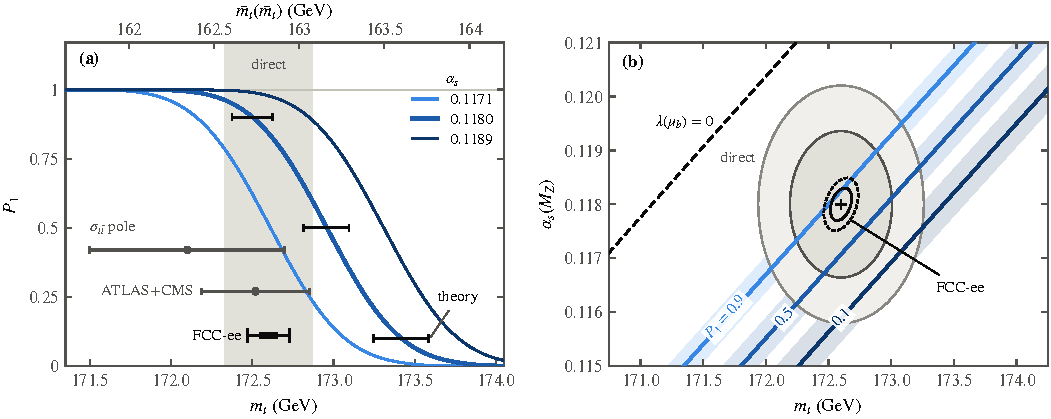
\includegraphics[width=\textwidth]{prd_criterion}
\caption{Top-mass criterion for survival.
(a)~Single-branch survival probability $\Pone(m_t)$ for $\alpha_s(M_Z)=0.1171$, $0.1180$ (thick), and $0.1189$, with theory $1\sigma$ bars (model, Standard Model mapping, $M_h$) at $\Pone=0.9$, $0.5$, and $0.1$.
Gray band: direct measurement; bars: $\sigma_{t\bar t}$ pole mass, ATLAS+CMS, and FCC-ee projection (thick: $m_t$; thin: total). %
Upper axis: $\mtbar$ at $\alpha_s=0.1180$.
(b)~Critical lines in the $(m_t,\alpha_s)$ plane with theory bands, the line $\lambda(\mub)=0$ (dashed), about $\mcMinusMzero\GeV$ below $\Pone=1/2$ (the absolute-stability line lies $0.10\GeV$ below it in $m_t$, Sec.~\ref{sec:rb-absstab}), and the $68\%$ and $95\%$ regions of present data and FCC-ee.} %
\label{fig:rb-criterion}
\end{figure}

\subsection{The absolute-stability line and the relative criterion}
\label{sec:rb-absstab}

The criterion is a statement about $\lambda$ at one scale, $\mub$, whereas the familiar stability bounds of the Standard Model concern the whole range of $\lambda(\mu)$.
To place it among them we computed, for this report, the absolute-stability line of the same mapping: the top pole mass $m_{\rm stab}$ at which
\begin{equation}
\min_{\mu\le\MPbar}\lambda(\mu)=0,
\label{eq:rb-absstab-def}
\end{equation}
with $\alpha_s(M_Z)=0.1180$ and $M_h=125.13\GeV$. %
The script \nolinkurl{higgs/01_sm_mapping/abs_stability.py} of the code package~\cite{DNECv12code} calls the Standard Model mapping of the main calculation, locates the minimum of $\lambda(\mu)$ on a logarithmic grid between $10^{8}\GeV$ and $\MPbar$, refines it with a bounded one-dimensional minimization in $\log_{10}\mu$, and solves for $m_{\rm stab}$ and $m_0$ with Brent's method; it writes \nolinkurl{abs_stability.json} next to itself.
We find
\begin{equation}
m_{\rm stab}=170.99\GeV\quad\bigl[\mtbar=161.29\GeV\bigr],\qquad m_0-m_{\rm stab}=0.10\GeV, %
\label{eq:rb-mstab}
\end{equation}
with the minimum of $\lambda(\mu)$ at $\mu=5.1\times10^{17}\GeV$, below $\MPbar$; the cut at the non-reduced Planck mass gives the same value. %
The script reproduces $m_0=171.0921\GeV$ (R5-029) to $2\times10^{-5}\GeV$ and $\lambda(\mub)$ at the central inputs to $4\times10^{-8}$, and a rerun with the research copy of the mapping gives identical values. %
At $\alpha_s=0.1171$ and $0.1189$ the line moves to $170.64$ and $171.34\GeV$, with $m_0-m_{\rm stab}=0.11$ and $0.09\GeV$. %
This number appears only in this report; the papers state only that the absolute-stability bound lies just below $m_0$~\cite{v12PRD,v12PRL}.

The ordering is therefore
\begin{equation}
m_{\rm stab}=170.99<m_0=171.09<m_c(\Pone=\tfrac12)=172.96\ll m_{\rm meta}=177.7\ \ {\rm GeV}, %
\label{eq:rb-ordering}
\end{equation}
where $m_{\rm meta}$ is the metastability bound of Ref.~\cite{Andreassen:2017rzq}, above which the electroweak vacuum of infinite flat space would have decayed in the age of the universe.
The finite-volume criterion lies $\mcMinusMzero\GeV$ above the line where $\lambda(\mub)$ changes sign and far below the metastability bound: a slightly negative quartic at $\mub$ is harmless, because the gauge zero-point energy confines the zero mode for the short duration of the turn. %
With our SMDR-type matching at the inputs of Ref.~\cite{Bednyakov:2015sca}, $M_h=125.7\GeV$ and $\alpha_s(M_Z)=0.1185$, the same script gives $171.47\GeV$, against $171.453\GeV$ with their own matching (Sec.~\ref{sec:rb-sm-bench}); the difference measures the matching scheme. %
In the relative form $m_c-m_0$ the criterion carries mainly the model error, because a shift of $\lambda(\mub)$ from the Standard Model mapping moves $m_c$ and $m_0$ together.

\subsection{Benchmarks and the change relative to fitted formulas}
\label{sec:rb-sm-bench}

From the matching formulas of Ref.~\cite{Buttazzo:2013uya} our running reproduces their couplings at the Planck scale: $g_1=0.61537$, $g_2=0.50546$, $g_3=0.48731$, $y_t=0.38245$, and $\lambda=-0.01436$, against $0.6154$, $0.5055$, $0.4873$, $0.3825$, and $-0.0143$. %
From the matching of Ref.~\cite{Bednyakov:2015sca} and for their inputs, $M_h=125.7\GeV$ and $\alpha_s(M_Z)=0.1185$, it reproduces their stability bound, $171.453\GeV$ at $\log_{10}(\mu/{\rm GeV})=17.750$ against $171.44\GeV$ and $17.752$. %
Two inputs of the fitted formulas differ from the full calculations.
The fitted $g_3(m_t)$ is $0.0017$--$0.0018$ higher than pure four-loop QCD, SMDR, and Ref.~\cite{Bednyakov:2015sca}, equivalent to $\Delta\alpha_s(M_Z)\approx+0.0004$, and the fitted $y_t(m_t)$ lacks the four-loop QCD term of the pole mass and is $0.00094$ too high. %

\begin{table}[t]
\centering
\caption{Change of the critical top mass at $\Pone=1/2$ when the earlier mapping (fitted matching, two-loop running, and a constant three-loop calibration of $\lambda$) is replaced by the mapping of this section, at $(m_t,\alpha_s)=(172.60\GeV,0.1180)$, converted with $d\lambda(\mub)/dm_t$.} %
\label{tab:rb-smchain}
\begin{tabular}{lcc}
\toprule
Step & $\lambda(\mub)$ & $\Delta m_c$ [GeV] \\
\midrule
Earlier mapping & $-0.0101929$ & \\ %
Five-loop running, no calibration & $-0.0103040$ & $-0.017$ \\ %
$g_3(m_t)$ from QCD & $-0.0110499$ & $-0.113$ \\ %
Four-loop QCD in $y_t(m_t)$ & $-0.0097062$ & $+0.203$ \\ %
SMDR matching & $-0.0097741$ & $-0.010$ \\ %
\midrule
Total & & $+0.063$ \\ %
\bottomrule
\end{tabular}
\end{table}

Table~\ref{tab:rb-smchain} decomposes the change relative to the earlier mapping.
The two corrections of the fitted inputs partly cancel, and the total, $+0.063\GeV$, is the same at all three levels of $\Pone$ to $0.002\GeV$ because the critical quartic at $\mub$ does not change. %
This is the step labelled NNLO in the refinement table of Sec.~\ref{rep:h-budget}.

\subsection{Top-mass definitions}
\label{sec:rb-mt-def}

With the same four-loop relation that enters the matching, the criterion reads $\mtbar<162.73$, $163.16$, and $163.60\GeV$ for $\Pone=0.9$, $0.5$, and $0.1$ at $\alpha_s(M_Z)=0.1180$, and $162.92$ and $163.41\GeV$ at $\Pone=1/2$ for $\alpha_s=0.1171$ and $0.1189$. %
The $\alpha_s$ dependence is $273\GeV$ per unit for $\mtbar$ against $387\GeV$ for the pole mass, about $30\%$ smaller, because part of the $\alpha_s$ dependence of $y_t(m_t)$ sits in the pole--$\MSbar$ relation. %
The $\mtbar$ form is free of the truncation of the pole series and of the renormalon ambiguity: the all-orders pole mass lies $0.272\GeV$ above our four-loop truncation, with an ambiguity of $0.07$--$0.11\GeV$~\cite{Beneke:2016cbu}. %

Top-mass definitions enter at the level of $0.5\GeV$~\cite{Butenschoen:2016lpz,Hoang:2020iah}. %
With the identification of assumption (A7), the direct (Monte Carlo) mass, $172.60\pm0.27\GeV$~\cite{ParticleDataGroup:2026mpi}, gives $\Pone=0.843$ at its central value. %
The cross-section pole mass, $172.1\pm0.6\GeV$~\cite{ParticleDataGroup:2026mpi}, gives $\Pone=0.99$, and the ATLAS+CMS combination, $172.52\pm0.33\GeV$~\cite{ATLAS:2024dxp}, gives $0.89$. %
For the direct mass we follow Ref.~\cite{Hoang:2020iah}: either it is identified with the pole mass with an interpretation error of $0.5\GeV$, or it is identified with the MSR mass at $1.3\GeV$, which lies $0.36\pm0.25\GeV$ below the pole mass~\cite{Hoang:2017suc}. %
Calibrations of the Monte Carlo against $e^+e^-$ event shapes support an interpretation error of this size~\cite{Butenschoen:2016lpz}.
The MSR identification puts the measured direct mass at a pole-mass equivalent of $172.96\GeV$, at the criterion itself, and gives $\Pbar=\PbarMSR$ (Sec.~\ref{rep:h-budget}). %

\subsection{Theory error of the mapping}
\label{sec:rb-sm-error}

The matching-scale dependence is the leading theory error, and three ways of estimating it differ by an order of magnitude.
(i)~Varying all evaluation scales of the compiled SMDR fit together by factors $\frac12$ and $2$ moves $m_c$ by $+0.033$ and $-0.019\GeV$. %
This small value comes from a cancellation: the top-mass scale alone gives $+0.067$ and $-0.027\GeV$, and the Higgs-mass scale $-0.037$ and $+0.011\GeV$. %
At two-loop accuracy for $M_h$ the Higgs-mass term doubles, to $-0.070$ and $+0.030\GeV$, while the common variation shrinks to $+0.006$ and $+0.002\GeV$, so the smallness reflects cancellation rather than convergence. %
Varying each scale independently gives the envelope $[-0.069,+0.082]\GeV$. %
(ii)~The two-loop fixed-order matching in the $G_F$ scheme~\cite{Bednyakov:2015sca,Kniehl:2016enc}, recomputed blind with the library mr, moves $m_c$ by $+0.173\GeV$ for $\mu_0=m_t/2$ and $-0.358\GeV$ for $\mu_0=2m_t$, reproducing the published scale variation of the stability bound. %
Decomposed linearly, $y_t$ contributes $+0.136/-0.196\GeV$, of which the pure-QCD tower is $+0.055/-0.066\GeV$, and $\lambda$ contributes $+0.037/-0.162\GeV$; the gauge couplings contribute less than $0.004\GeV$. %
In that scheme the non-QCD logarithms of $\lambda$ and $y_t$ are large and of the same sign; they, and not the tadpoles, cause the larger spread, since the tadpole contributions cancel identically in the coefficients used there.
(iii)~A reconstruction of the missing three-loop logarithms from the renormalization group, which we used before compiling SMDR, gives $[-0.088,+0.102]\GeV$ and overestimates the full calculation by about a factor of three. %

We adopt the following budget.
For the matching scale we take the independent variation of the SMDR evaluation scales, with the pure-QCD tower removed from the top-mass scale, $[-0.042,+0.054]\GeV$; it does not rely on the cancellation of (i). %
For the organization of the fixed-order result we take the difference between mr and SMDR at $\mu_0=m_t$, $0.042\GeV$, a direct calculation that includes the leading three-loop terms of SMDR ($0.014\GeV$). %
The truncation of the running ($0.005\GeV$), the order of the $\alpha_s$ input ($0.003\GeV$), and the $W$ and $Z$ pole-mass convention ($0.011\GeV$) are small. %
In quadrature these give $\pm0.070\GeV$ for $\mtbar$. %
The pole form adds $0.075\GeV$ for the uncomputed $O(\alpha_s^5)$ term of Eq.~(\ref{eq:rb-zm}), a geometric extrapolation that agrees with the scale variation of the pure-QCD tower and with the renormalon ambiguity; these are the same order and are counted once. %
The total for the pole form is $\pm0.102\GeV$. %
The $G_F$-scheme spread of (ii), $+0.17/-0.36\GeV$ in $m_c$, enters only as a robustness variant, with $\Pbar=\PbarBKPV$ depending on how its asymmetric errors are combined (Sec.~\ref{rep:h-budget}). %

The parametric errors are kept separate.
$M_h=125.13\pm0.11\GeV$ moves $m_c$ by $\pm0.053\GeV$, and $\alpha_s(M_Z)=0.1180\pm0.0009$ by $\pm0.35\GeV$ ($\pm0.25\GeV$ for $\mtbar$). %
Using $M_h=125.20\GeV$ instead would raise $m_c$ by $0.034\GeV$. %
The scale variation estimates the three-loop electroweak and mixed threshold corrections at $\mu_0$.
Assumption (A2) takes the Standard Model to hold up to $\mub$; new states below $\mub$ that couple to the Higgs would change $\lambda(\mub)$, and the criterion tests the Standard Model up to that scale.

\subsection{Independent mapping}
\label{sec:rb-sm-blind}

An independent mapping was written from the published conventions alone, without access to our code, using mr~1.3.2~\cite{Kniehl:2016enc} for the matching and its three-loop $\beta$ functions (Sec.~\ref{rep:v-blind}).
Its 276 three-loop monomials agree with the appendix of Ref.~\cite{Buttazzo:2013uya} one by one, and numerically with the SMDR $\beta$ functions to $10^{-15}$. %
With the SMDR matching its quartic at $\mub$ differs from ours by $4\times10^{-6}$, equivalent to $0.0006\GeV$, and its $y_t$ by $2\times10^{-6}$. %
With the mr matching it is lower by $2.8\times10^{-4}$, or $0.043\GeV$, which is the scheme item of the budget. %
The library mr must run single-threaded; its OpenMP sections otherwise give nondeterministic two-loop integrals.
The blind check also compiled SMDR independently and reproduced our scale variations of (i) exactly, so the differences between (i) and (ii) are traced to their source and not to an implementation.
